\documentclass[10pt,twocolumn,letterpaper]{article}

\usepackage{aicourse}
\usepackage{times}
\usepackage{epsfig}
\usepackage{graphicx}
\usepackage{amsmath}
\usepackage{amssymb}

% Include other packages here, before hyperref.

% If you comment hyperref and then uncomment it, you should delete
% egpaper.aux before re-running latex.  (Or just hit 'q' on the first latex
% run, let it finish, and you should be clear).
\usepackage[breaklinks=true,bookmarks=false]{hyperref}


\aicoursefinalcopy


\setcounter{page}{1}
\begin{document}


%%%%%%%%%%%%%%%%%%%%%%%%%%%%%%%%%%%%%%%%%%%%%%%%%%%%%%%%%%%%%%%
% DO NOT EDIT ANYTHING ABOVE THIS LINE
% EXCEPT IF YOU LIKE TO USE ADDITIONAL PACKAGES
%%%%%%%%%%%%%%%%%%%%%%%%%%%%%%%%%%%%%%%%%%%%%%%%%%%%%%%%%%%%%%%



%%%%%%%%% TITLE
\title{\LaTeX\ ECS7036P - An AI Approach to Running Route Optimisation for Safety}

\author{David Shafirovich\\
200349804\\
{\tt\small d.j.shafirovich@se25.qmul.ac.uk}
\and
Hongyuan Zhai\\
260019183\\
{\tt\small h.zhai@se25.qmul.ac.uk}
\and
Raena Fadzil\\
250988321\\
{\tt\small r.fadzil@se25.qmul.ac.uk}
}


\maketitle
%\thispagestyle{empty}



% MAIN ARTICLE GOES BELOW
%%%%%%%%%%%%%%%%%%%%%%%%%%%%%%%%%%%%%%%%%%%%%%%%%%%%%%%%%%%%%%%


%%%%%%%%% ABSTRACT
\begin{abstract}
   The abstract for your project goes here. The length of the abstract should be between 200-250 words. Tips for writing a good abstract can be found at \url{https://qmplus.qmul.ac.uk/mod/book/view.php?id=3310704&chapterid=323502}.
   
Can personal safety be treated as a primary objective in pedestrian route planning, rather than an afterthought to distance and time? Mainstream running and navigation apps optimise almost entirely for speed, leaving solo runners, especially after dark, to judge safety for themselves. This project addresses that gap by building and deploying a safety-first, lighting-aware routing tool for the London Borough of Camden. 

On the data side, open records of crime, stop-and-search, and street lighting are attached to an OpenStreetMap street graph at the level of individual streets. Each crime is scored in two complementary ways, by legal severity and by perceived risk, drawing on the Cambridge Crime Harm Index and the Signal Crimes Perspective, and its influence is spread along the walkable network using a Network-Based Kernel Density Estimate that respects the anonymised resolution of the police data.

\textbf{<PLACEHOLDER - David’s input on the model>} 

\textbf{<PLACEHOLDER - Rae’s input on the routing integration and front-end>}

\textbf{<PLACEHOLDER - headline evaluation result>} 

The result is a working prototype showing that data-driven safety routing is feasible and practically useful for everyday runners.

\end{abstract}

%%%%%%%%% BODY TEXT
\section{Introduction}

Running participation in the UK has grown steadily in recent years, and events such as the London Marathon now attract record numbers of applicants. Running is one of the most accessible forms of exercise, requiring no gym membership or specialist equipment, and is widely recognised for its mental health benefits alongside its physical ones. Existing running and journey-planning apps, however, optimise almost exclusively for distance or time. Neither category of app treats personal safety as a crucial routing objective, despite safety being a commonly cited concern for solo runners, after dark or in unfamiliar cities.

This project addresses that gap by building a safety-first and street-lighting-aware pedestrian routing tool, scoped to the London Borough of Camden as a case study. The system attaches risk-related features derived from open crime, stop-and-search, and street lighting data to a street-level graph, trains a predictive model on that history, and injects the resulting risk estimates directly into a production-grade routing engine (Valhalla) so that riskier streets are naturally avoided where a reasonable alternative exists. A companion lighting indicator, based on current streetlight coverage rather than a trained prediction, is shown alongside each route for the user's own judgement, particularly relevant for evening use.

The remainder of this report describes prior work in safety-aware routing (Section 2), the data pipeline, predictive model, and routing integration that were actually built (Section 3), the datasets, software, and hardware involved (Section 4), the current state of evaluation together with an honest account of what remains outstanding against the project proposal (Section 5), and our conclusions and remaining contributions (Sections 6-8).

\section{Related Work}

A small but growing body of work treats safety as an explicit navigation objective rather than a secondary constraint. Atterkar et al.~\cite{atterkar2025womensafe} propose a Women Safe Route Navigation System that scores streets by risk and steers users away from higher-risk areas. Harideviprathap et al.~\cite{harideviprathap2026mogat} extend this with Mo-GAT, a multi-objective spatiotemporal graph attention network that predicts safety risk across a street network and adapts as conditions change over space and time. Anson~\cite{anson2025mlrouting} studies how a machine-learned weighting of a road network can be consumed by a path-finding algorithm in a smart urban transport setting, which is architecturally close to the approach this project ultimately takes. Tang et al.~\cite{tang2024itinera} pair spatial optimisation with large language models to plan open-ended urban itineraries, demonstrating that data-driven, objective-aware routing is achievable at city scale.

These studies establish that safety-first, data-driven routing is both feasible and an active research area, but each targets either a specific demographic-focused safety application or a general urban commuting/itinerary-planning use case. None specifically targets the everyday runner, and none of the mainstream commercial running or journey-planning applications currently used by the public (Section 1) incorporate a safety objective at all. This project sits between these two spaces: applying a data-driven safety model, in the spirit of \cite{atterkar2025womensafe,harideviprathap2026mogat}, but integrated directly into a general-purpose, open-source routing engine rather than a bespoke path-finding implementation.

\section{Proposed Method}

\subsection{Data Pipeline}

The first stage is a data pipeline that turns raw open data into a table with one row per street segment. A pedestrian street graph for Camden i downloaded from OpenStreetMap via OSMnx~\cite{boeing2017osmnx}, giving 35{,}532 edges. Onto it we attach three open datasets at edge level: recorded crime and stop-and-search from the UK Police API~\cite{datapoliceuk2026}, and street lighting from Camden Council~\cite{camden2026lighting}. Crime is pulled month by month; since data.police.uk only keeps a rolling window, the pipeline clips the request to whatever is actually published at run time, here 36 months from June 2023 to May 2026.

We compute two crime weightings per incident, since since ``serious'' and ``frightening'' differ. A \emph{severity} score (1--3) follows the Cambridge Crime Harm Index~\cite{sherman2016cambridge} and the ONS Crime Severity Score~\cite{ons2016severity}; a separate \emph{perceived risk} score (1--4) follows the Signal Crimes Perspective~\cite{innes2004signal,innesfielding2002signal} and ONS survey data~\cite{ons2022csew}, under which visible disorder can outweigh a legally more serious but less visible offence. Each edge's score is the sum of its incidents' weights. Both are deliberate simplifications onto the 14 categories the API exposes, not a full reproduction of either study.

Police coordinates are anonymised to fixed snap points roughly 125\,m apart in Camden, so assigning a crime to one nearest street would be misleadingly precise. Instead each incident's weight is spread over nearby streets using Network Kernel Density Estimation~\cite{chainey2008hotspot}, with distance measured \emph{along} the walkable graph (Dijkstra shortest paths) rather than in a straight line, so a crime cannot bleed across a wall or the canal. The bandwidth is set to 125\,m to match the anonymisation spacing, and smoothing is done separately per month so future data cannot leak into earlier months.

The pipeline outputs two tables. \texttt{edge\_features.csv} holds the crime and stop-and-search features (overall totals, a per-month breakdown, and the per-month NetKDE columns used by the model); \texttt{edge\_lamp\_features.csv} holds the lighting features separately, as lighting is a current snapshot with no monthly history. Both carry the OpenStreetMap way ID and endpoint coordinates so any row traces back to a real place. After cleaning, the dataset holds 230{,}707 crimes, 24{,}644 stop-and-search records, and 15{,}561 lamps. Stop-and-search gender, age, and ethnicity fields were deliberately excluded to avoid encoding demographic bias into a safety score.

\subsection{Predictive Safety Model}

\textbf{<PLACEHOLDER - David to review/edit>}

\subsection{Notes}

\subsubsection{Model Architecture \& Objective}
\begin{itemize}
    \item \textbf{System:} The system uses an XGBoost Regressor (\texttt{xgb.XGBRegressor}).
    \item \textbf{Objective Function:} The primary objective function is \texttt{reg:squarederror}, as the model is designed to predict continuous float values representing the NetKDE Perceived Risk score of a street.
\end{itemize}

\subsubsection{Hyperparameter Configuration}
\begin{itemize}
    \item \textbf{Number of Trees:} 500 (\texttt{n\_estimators}).
    \item \textbf{Learning Rate:} 0.05.
    \item \textbf{Tree Depth:} Maximum depth of 6.
    \item \textbf{Sampling:} Both \texttt{subsample} and \texttt{colsample\_bytree} are set to 0.8 to prevent overfitting.
    \item \textbf{Categorical Handling:} Natively enabled (\texttt{enable\_categorical=True}) for features like highway types.
    \item \textbf{Early Stopping:} Set to 50 rounds to halt training if validation performance stops improving.
\end{itemize}

\subsubsection{Training \& Evaluation Strategy}
\begin{itemize}
    \item \textbf{Chronological Split:} The dataset is split sequentially, using a cutoff month (March 2026) to train on past historical data and test strictly on future data.
    \item \textbf{Data Masking:} Raw identifiers (e.g., \texttt{osmid}, \texttt{edge\_id}, \texttt{name}) and current-month crime totals are dropped to prevent the model from learning raw IDs or experiencing target leakage.
    \item \textbf{Evaluation Metric:} The model's predictive accuracy is evaluated using Mean Absolute Error (MAE) on the future test set.
    \item \textbf{Interpretability:} Feature importance is calculated and plotted using ``Information Gain'' to determine which variables have the highest predictive power.
\end{itemize}

\subsubsection{Input Features}
\begin{itemize}
    \item \textbf{Historical Lags:} Relies on spatial-temporal lag features, specifically 2, 3, and 4-month historical lags for NetKDE perceived risk and stop-and-search counts.
    \item \textbf{Static Metadata:} Incorporates street-level characteristics including start/end coordinates (\texttt{u\_lat}, \texttt{v\_lng}, etc.), street length, and highway category.
    \item \textbf{Lighting Data:} Feeds on static environmental variables like \texttt{lamp\_per\_km} and \texttt{is\_lit}.
\end{itemize}

\subsubsection{Output Generation \& Routing Integration}
\begin{itemize}
    \item \textbf{Baseline Predictions:} The model predicts a raw future safety score, with predictions clipped at a lower bound of 0.
    \item \textbf{Cost Scaling:} The raw predictions undergo a logarithmic transformation (\texttt{log1p}), followed by min-max scaling to convert them into a standardized 1 to 10 ``Safety Cost'' scale.
    \item \textbf{Mapping:} The final 1--10 integer values are mapped back to OpenStreetMap (OSM) nodes and edges as safety tags, which are then used as penalty weights by the routing algorithm to calculate the safest daytime and nighttime paths.
\end{itemize}
The project proposal considered two candidate architectures: an XGBoost binary classifier feeding an A* search, and a graph attention network (GAT) predicting risk directly over the street network.

What was implemented is an XGBoost \emph{regressor} that forecasts future crime-related risk density at street level. The wide-format monthly dataset is restructured into a long-format panel (one row per street segment per month), and temporal lag features (1-, 2-, and 3-month lookbacks, grouped strictly by street segment) give the model historical context. All-time cumulative columns and same-month target metrics are deliberately excluded from the feature set to prevent data leakage. The data is split chronologically, training on historical months and validating on a held-out future period, rather than using a random split, since a random split would let future information leak into training.

To generate a forward-looking risk estimate, the most recent available month's data is shifted forward to serve as the new one-month lag, and the model's predicted crime count is converted to a density (predicted count divided by street length). This density is min-max scaled into an ordinal \texttt{safety\_tag\_value} from 1 (baseline) to 11 (highest risk), written to \texttt{osm\_safety\_tags.csv} keyed by OpenStreetMap way ID. A minimum tag value is enforced so that no street receives a zero-cost weighting downstream. Node-level aggregation was deliberately not used, since Valhalla's routing costing requires continuous per-edge penalties to discourage travelling \emph{down} a dangerous street, not merely arriving at a risky junction.

\subsection{Routing Integration}

Rather than implementing a custom path-finding algorithm, the risk tags produced by the model are converted into cost multipliers and supplied to Valhalla~\cite{valhalla2026}, an open-source routing engine, via its native \texttt{linear\_cost\_factors} request parameter. Each flagged street's multiplier is computed as
\[
\text{multiplier} = 1 + \text{SCALE} \times (\text{tag} - 1),
\]
where SCALE is a single tunable constant. Streets at the baseline tag (the large majority of the network) receive no multiplier and are omitted from the request entirely, keeping each request small. Valhalla's existing shortest-path search then naturally prefers routes that avoid heavily-multiplied streets where a reasonable detour exists, while still permitting a short traversal of a risky street when no reasonable alternative is available, since the engine is minimising a distorted notion of distance rather than obeying a hard exclusion rule.

\subsubsection*{Safety Score}
A separate, purely descriptive \textbf{safety score} (0-100) is computed \emph{after} routing, by measuring what proportion of a returned route's length passes within a fixed proximity radius of a flagged street; this score has no influence on which route is chosen; it exists to communicate, in an interpretable way, how much residual exposure a given route carries.

\subsubsection*{Lighting Indicator}
A second, independently displayed \textbf{lighting score} (0-100) reports what proportion of a route's length passes near a currently lit street, based directly on the raw lamp dataset rather than a trained forecast. It was deliberately kept out of the routing cost function and out of the automatic ``recommended route'' selection, so that the routing decision continues to optimise for the modelled safety objective alone; the lighting score is intended as an at-a-glance signal for the user's own judgement, particularly for evening or night-time use.

\section{Experiments}

\subsection{Dataset}
The street network, crime, stop-and-search, and lighting data are all scoped to the London Borough of Camden, extracted as an OpenStreetMap \texttt{.osm.pbf} file via the BBBike extract service~\cite{bbbike2026}. The dataset spans 36 monthly periods from June 2023 to May 2026, covering 35{,}532 street edges, 230{,}707 crime records, and 24{,}644 stop-and-search records. Records with missing or non-numeric coordinates and exact duplicate rows are removed during cleaning, and all coordinates are reprojected to the British National Grid to support metre-based distance calculations.

\subsection{Software}
The data pipeline uses Python with OSMnx~\cite{boeing2017osmnx}, GeoPandas, Shapely, pandas, and pyproj. The predictive model uses XGBoost. The routing engine is Valhalla~\cite{valhalla2026}, run inside Docker alongside a Python (FastAPI) proxy service that injects the safety cost factors into each routing request and computes the descriptive safety and lighting scores. The frontend is a React/MapLibre web application (adapted from Valhalla's own reference web app) presenting routes, scores, and turn-by-turn directions to the user.

\subsection{Hardware}
\textbf{<PLACEHOLDER>}

\section{Results and Discussion}

\textbf{<PLACEHOLDER>}

\textbf{<PLACEHOLDER - re. Routing UI>} The SCALE parameter controls a genuine trade-off: a street with a 4$\times$ multiplier is treated as roughly four times its real length, so the engine takes a detour only when a genuinely shorter alternative exists, whereas a street with a much higher multiplier (up to 31$\times$ at the highest observed risk tag during development) is avoided far more readily, but the engine will still traverse a short high-risk stretch rather than accept an extremely long detour, since it is minimising a distorted distance rather than applying a hard exclusion. A ``recommended route'' selection was also implemented on top of the three routes Valhalla returns per request: by default the fastest route is recommended, but if its descriptive safety score falls below a threshold, the fastest route within a 20\% time budget that clears the threshold is recommended instead.

Figures~\ref{fig:ui-screenshot-1} and~\ref{fig:ui-screenshot-2} are placeholders for screenshots of the working interface and should be replaced with real captures of the deployed application before submission.

\begin{figure}[t]
\begin{center}
   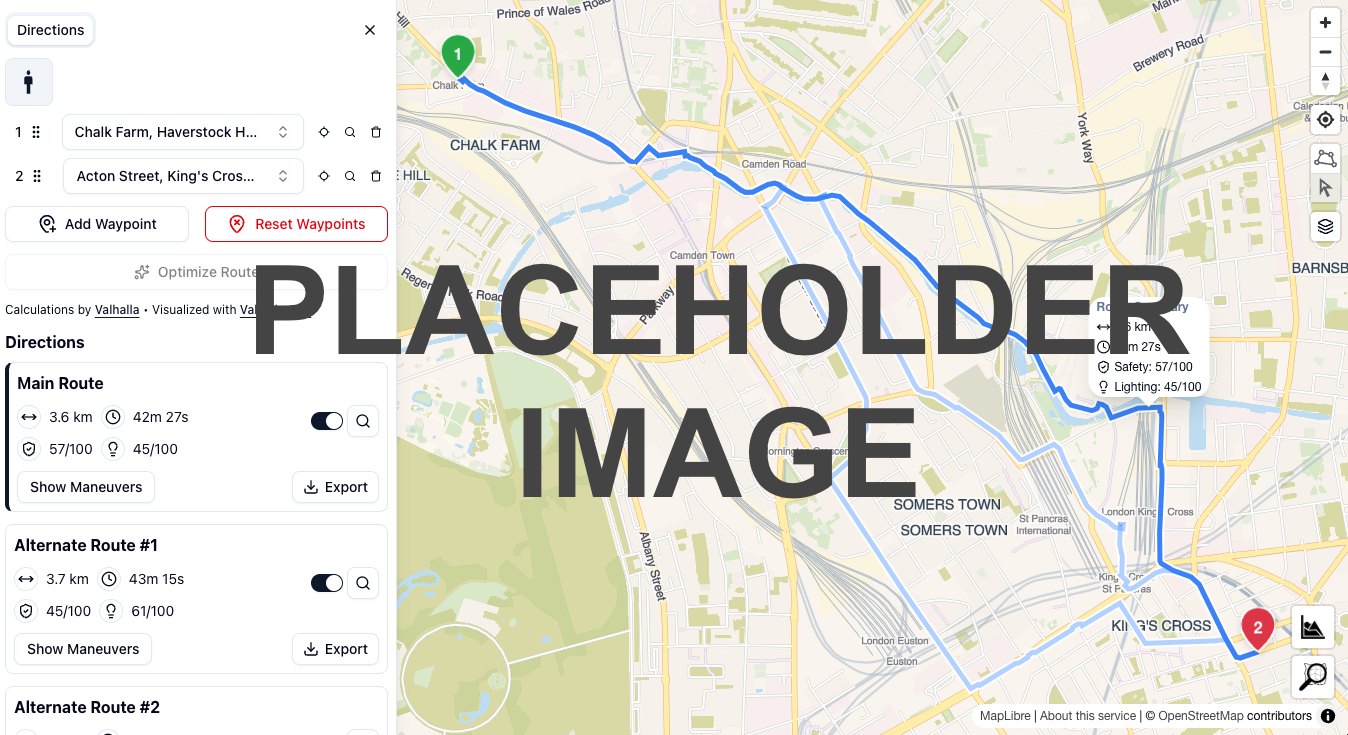
\includegraphics[width=0.8\linewidth]{figures/ui-screenshot-1.png}
\end{center}
   \caption{Placeholder - replace with a screenshot of the route summary panel, showing distance, time, safety score, and lighting score for a suggested route.}
\label{fig:ui-screenshot-1}
\end{figure}

\begin{figure}[t]
\begin{center}
   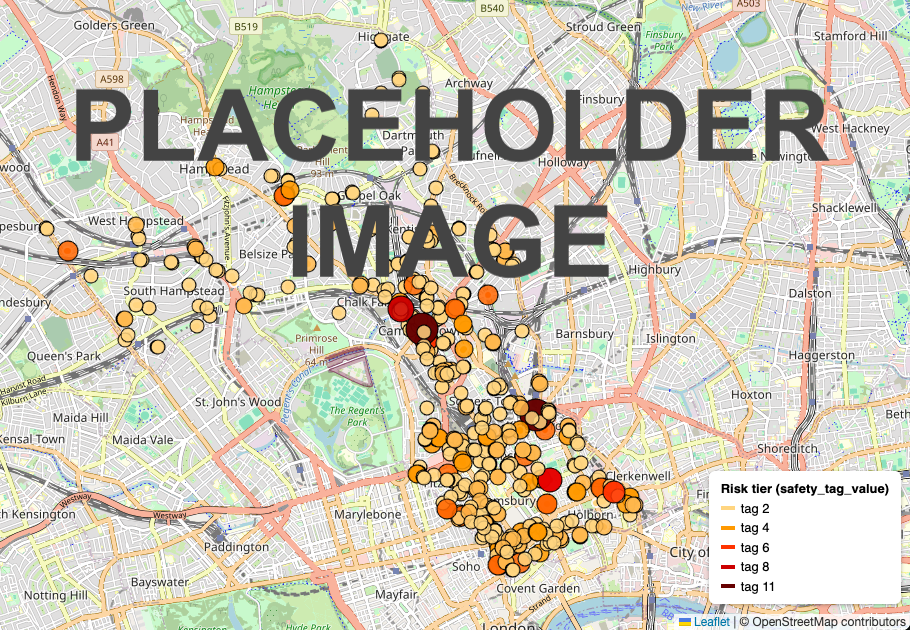
\includegraphics[width=0.8\linewidth]{figures/ui-screenshot-2.png}
\end{center}
   \caption{Placeholder - replace with a screenshot of the safety map viewer, showing flagged streets overlaid on the Camden street network.}
\label{fig:ui-screenshot-2}
\end{figure}

\section{Conclusions}

\textbf{<PLACEHOLDER - comparisons and evaluation>}
This project delivers a working, deployable prototype: a pedestrian router for Camden that prioritises safety, built by attaching a predictive crime-risk model's output to a production routing engine's native costing mechanism.

\section{Acknowledgements}

This project relies entirely on publicly available data and open-source software. We acknowledge OpenStreetMap and its contributors~\cite{osm2026}, the UK Police open data initiative~\cite{datapoliceuk2026}, the London Borough of Camden's open data portal~\cite{camden2026lighting}, the Valhalla routing engine and its contributors~\cite{valhalla2026}, and the BBBike extract service~\cite{bbbike2026}.
We thank Dr Anum Masood and Stephanie Keddy for their guidance and feedback throughout the project.

\section{Contributions}

The project proposal defined three lead roles:

\begin{itemize}
\item \textbf{Data Lead - Hongyuan Zhai:} Requirement analysis, and data collection, cleaning, and preparation.
\item \textbf{AI Model Lead - David Shafirovich:} AI problem formulation, model implementation, training, testing, and evaluation.
\item \textbf{Deployment Lead - Raena Fadzil:} front-end application development, model integration with the front-end, and stretch goals.
\end{itemize}

Each member led their own area as above and wrote the corresponding sections of this report. Where the components met, the feature pipeline into the model, and the model output into the routing engine, the work was shared, and all members reviewed the report for consistency.
Note: For rubric, refer to the Group Project Guidelines: \url{https://qmplus.qmul.ac.uk/mod/resource/view.php?id=3794535}

{\small
\bibliographystyle{ieee}
\bibliography{bibliography.bib}
}

\end{document}
